\section{Spektroskopie der Hyperfeinstruktur von Rubidium}
\subsection{Durchführung}
Bei der Messung des Hyperfein-Absorptionsspektrums befinden sich die beiden Linsen und
die Rubidiumzelle im Strahlengang.
Der Konstantanteil des Laserstroms, Modulationsamplitude und -frequenz
sind wie bei der Messung der Zeitabhängigkeit der Laserfrequenz (\autoref{sect:durchführung}).
Äußere Magnetfelder bleiben unkompensiert, weil die Zeeman-Aufspaltung der Hyperfeinstruktur im Erdmagnetfeld
mit der Linienbreite der Laserdiode nicht auflösbar ist.
Die Messung wird auf der steigenden und der fallenden Flanke der Modulationsspannung durchgeführt und
während der Messung wird die Zelle mit dem Föhn geheizt.


\subsection{Auswertung}
Da in dieses Teil der Auswertung häufiger Kurvenanpassungen mit einer Gauß-Funktion durchgeführt werden, wird folgende Konvention eingeführt:
\begin{equation}
    \label{eq:convention:gauss}
    \gaus(x; A, \mu, \sigma) := A \cdot e^{-\frac{1}{2} \left( \frac{x-\mu}{\sigma} \right)^2}
\end{equation}
\subsubsection*{Frequenzkalibrierung}
Das Etalonspektrum und die Spannung der Lasermodulation sind in \autoref{img:etalon:fit} abgebildet. 
Die Peaks des Etalonspektrums werden mit Cauchy-Kurven und einem linearen Untergrund gefittet. 
\begin{equation}
    U_\text{ph}(t) = a_\text{ph} + b_\text{ph} \cdot t + \frac{A}{\pi} \frac{s}{s^2 + (t-x)^2}
\end{equation}
Dabei ist das Zentrum $x$ und der Breiteparameter $s$.
Des Weiteren wird die Spannung für die Lasermodulation mit einer Geraden gefittet.
\begin{equation}
    U_\text{L}(t) = a_\text{L} + b_\text{L} \cdot t
\end{equation}
\begin{figure}[H]
\begin{center}
  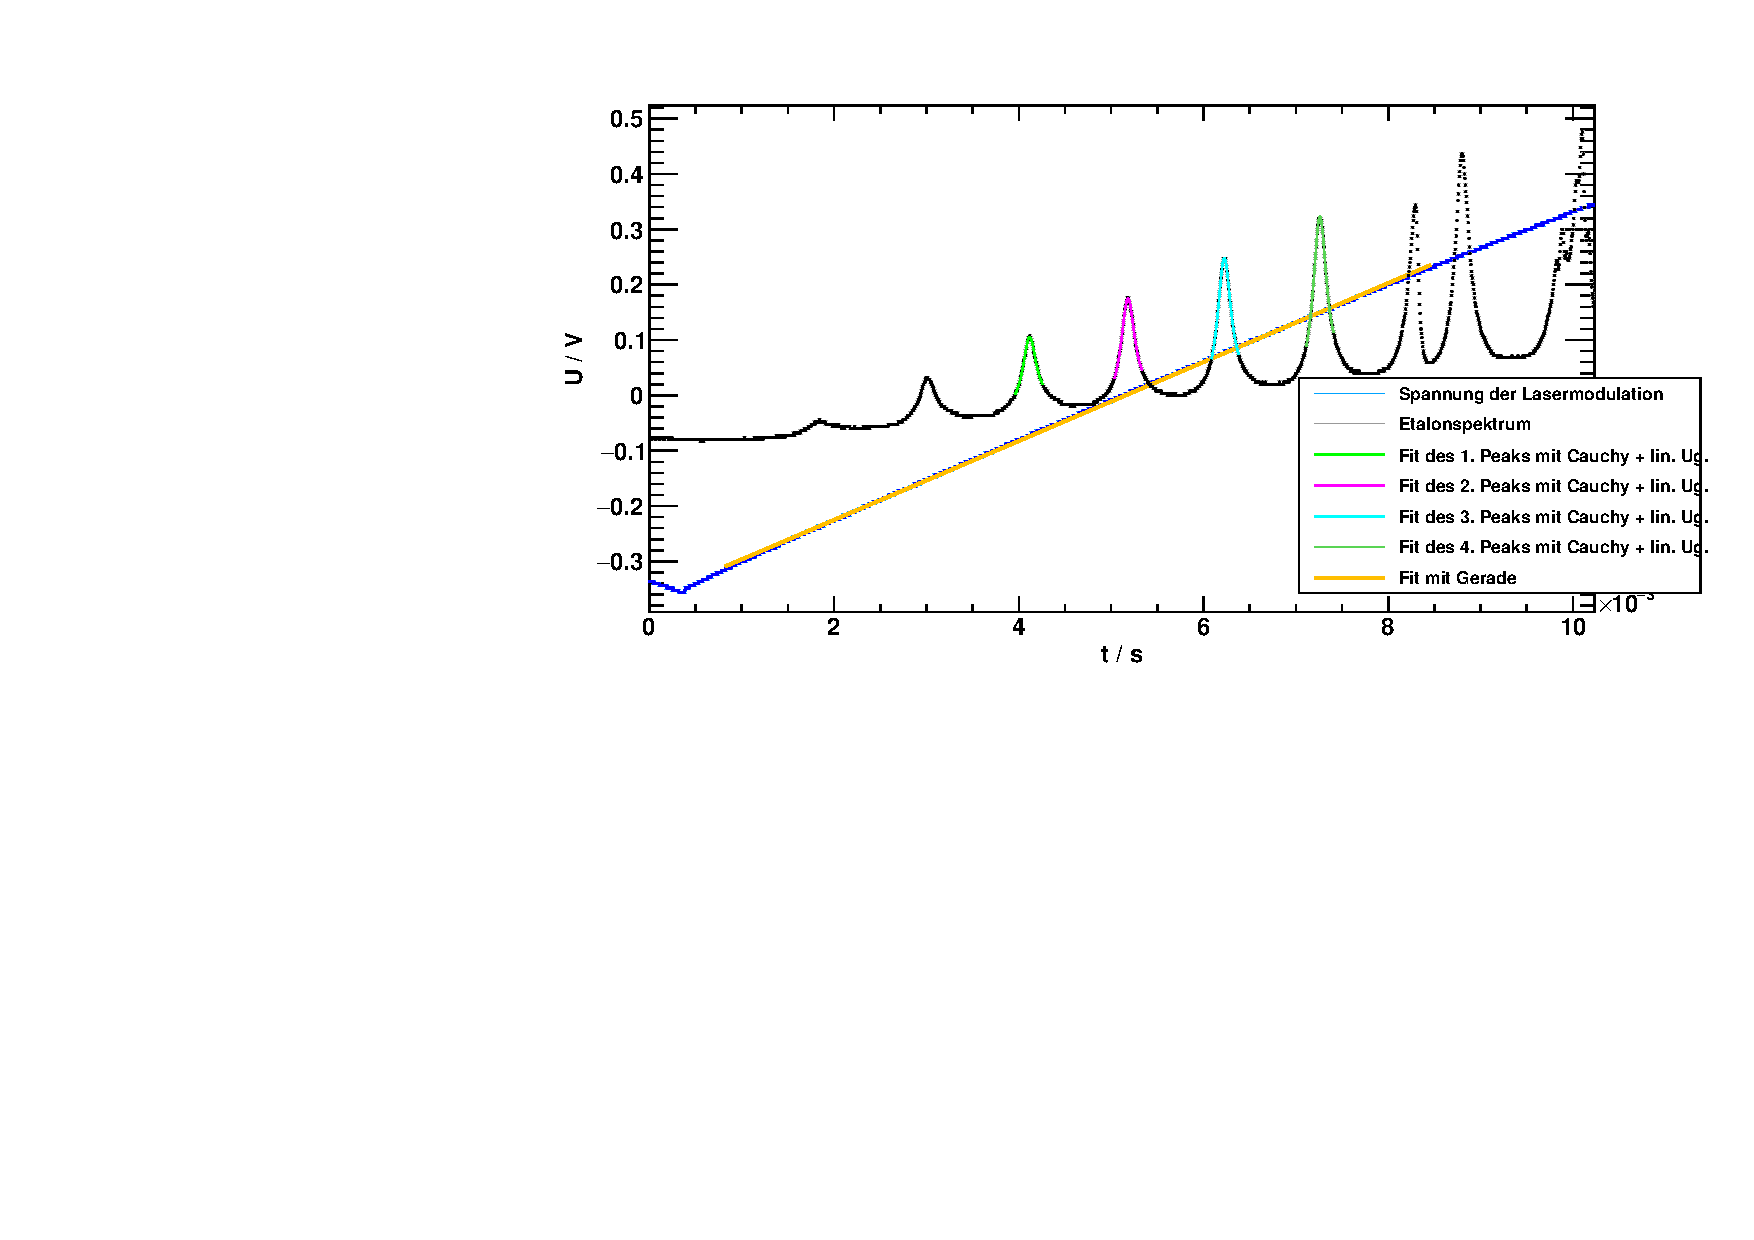
\includegraphics[width=\textwidth]{../img/part2/up-etalon_zoom_fit.pdf}
  \caption{caption.}
  \label{img:etalon:fit}
\end{center}
\end{figure}
Der Fit von $U_\text{L}$ kontrolliert, ob die Spannung für die Lasermodulation auch gerade ansteigt. Man erkennt, dass die angepasste Gerade 
gut der gemessenen Spannung folgt.\\
Aus dem freien Spektralbereich des Etalons $\Delta \nu_\text{FSR} = 9924 \pm 30\,\text{MHz}$ lässt sich nun die Differenz der Laserfrequenz von den verschiedenen 
Peaks bestimmen. Der erste Peak wird als Referenzpeak festgelegt. Der Frequenzabstand $\nu_i$ zwischen erstem und $i$-ten Peak lässt sich nun 
folgendermaßen berechnen\footnote{Gedankenspiel zur Fehlerrechnung: Interpretiert man $2 \cdot a$ als $a + a$, so ist der Fehler im ersten Fall $2 \cdot s_a$, im zweiten 
allerdings $\sqrt{2} \cdot s_a$, wenn man die Selbstkorrelation von $a$ nicht berücksichtigt. Mit $\cor(a, a) = 1$ 
erhält man $\sqrt{s_a^2 + s_a^2 + 2 \cdot s_a \cdot s_a \cdot \cor(a, a)} = 2 \cdot s_a$.}: 
\begin{equation}
    \Delta \nu_i = i \cdot \Delta \nu_\text{FSR}, \qquad s_{\Delta \nu_i} = i \cdot s_{\Delta \nu_\text{FSR}} 
\end{equation}
Die Frequenzabstände $\Delta \nu_i$ werden nun gegen die Zentren $x_i$  der 
Etalonpeaks aufgetragen (\autoref{img:etalon:calibration}). Da der Fehler der Zentren der Cauchy-Funktionen viel zu gering ist, wird der Fehler 
auf $\frac{1}{5}$ der Breiteparamter $s_i$ geschätzt. Die so berechneten Werte sind in \autoref{tab:etalon:calib:up} aufgelistet.
\begin{table}[H]
\caption{Zentren $x_i$ der gefitteten Cauchy-Funktionen mit abgeschätztem Fehler aus den Breiteparametern $s_i$ und Frequenzdifferenzen zum ersten Peak. }
\begin{center}
\begin{tabular}{|c|c|c|c|c|}
  \hline
  i & $x_i$ / s & $0.2 \cdot s_i$ / s & $\nu_i$ / GHz & $s_{\nu_i}$ / GHz \\ \hline
  1 & 4.117 & 0.018 & 0.00 & 0.00 \\ \hline
  2 & 5.181 & 0.018 & 9.92 & 0.03 \\ \hline
  3 & 6.225 & 0.018 & 19.85 & 0.06 \\ \hline
  4 & 7.260 & 0.018 & 29.77 & 0.09 \\ \hline
\end{tabular}
\end{center}
\label{tab:etalon:calib:up}
\end{table}


\begin{figure}[H]
\begin{center}
  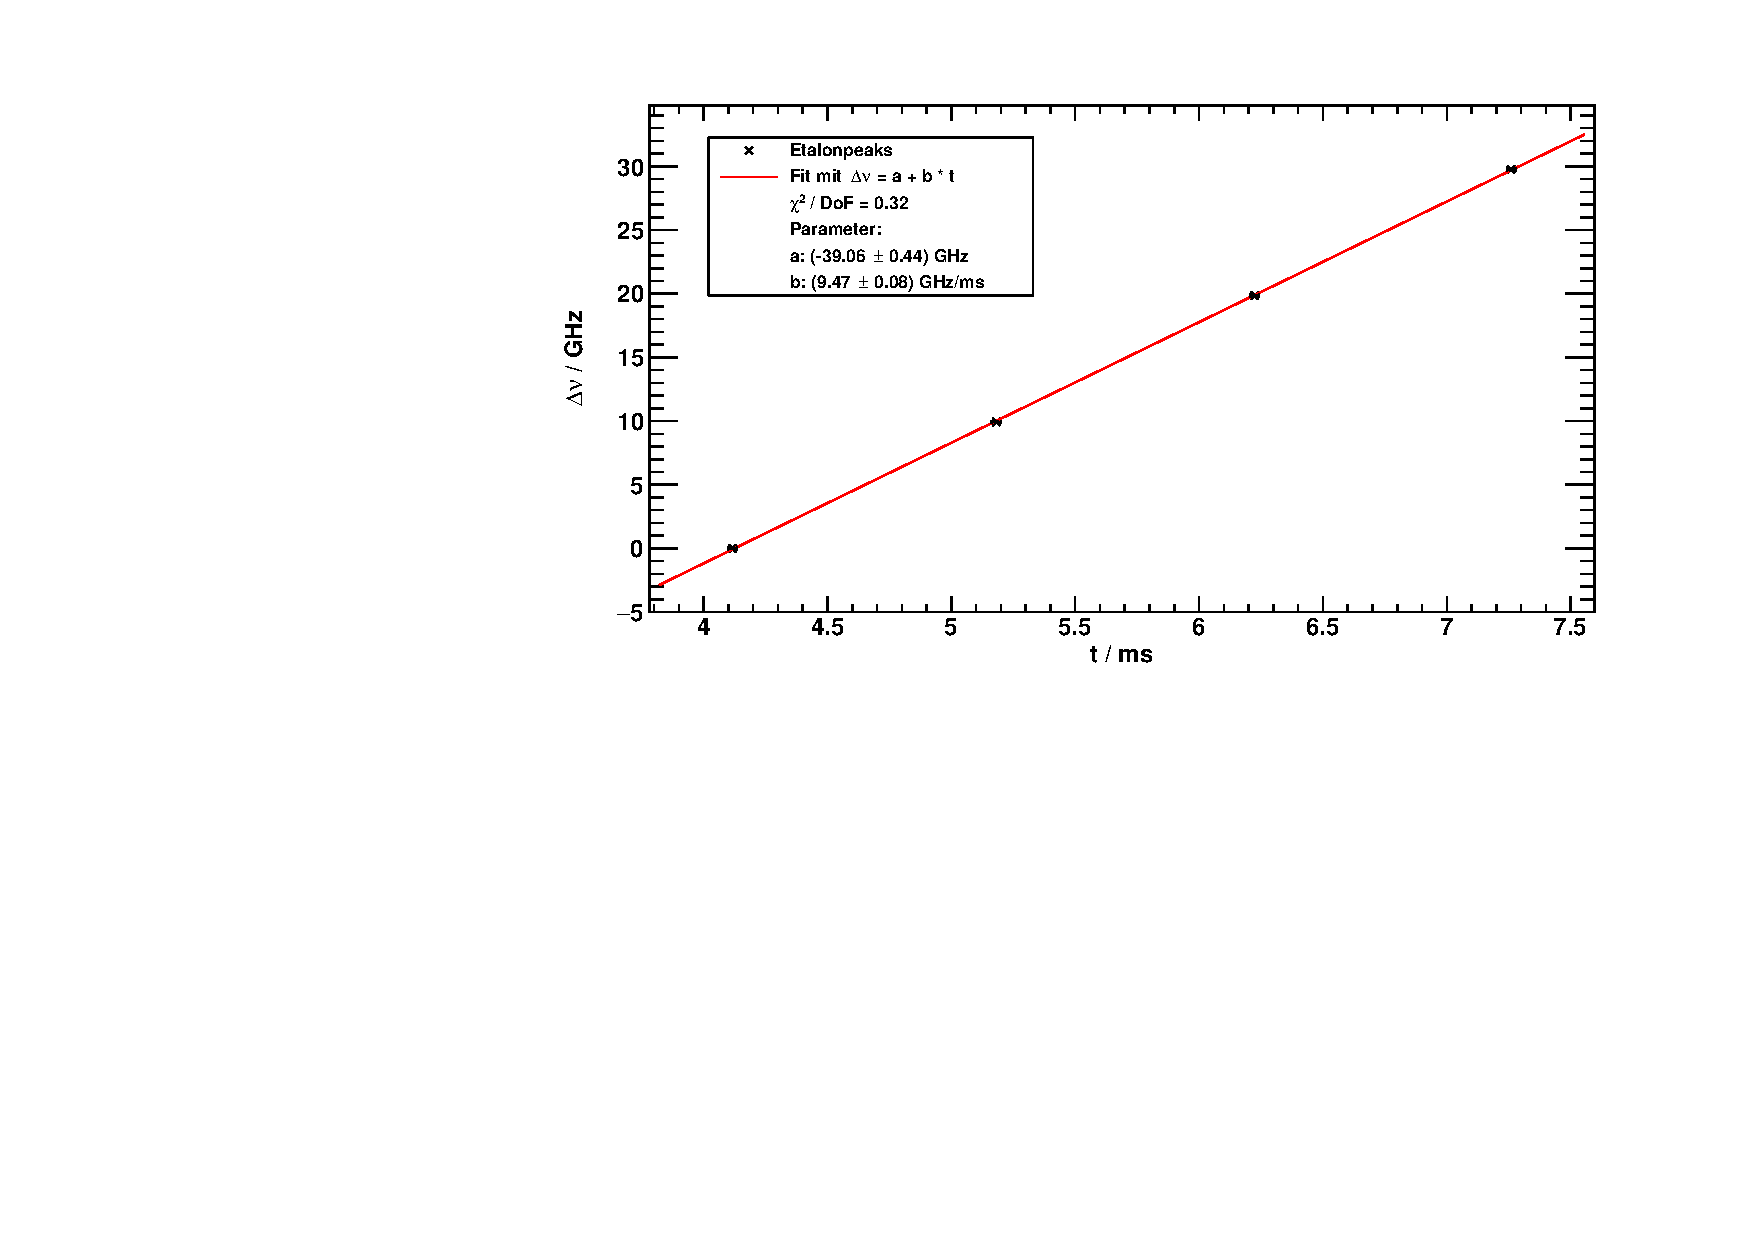
\includegraphics[width=\textwidth]{../img/part2/up-etalon_zoom-etalon_calibration.pdf}
  \caption{caption.}
  \label{img:etalon:calibration}
\end{center}
\end{figure}
Aus dem Fit mit einer Geraden 
\begin{equation}
    \Delta \nu(t) = a + r \cdot t  %TODO Parameter in Plot ändern
\end{equation}
lässt sich nun die Scanrate $r$ bestimmen. Man erhält %TODO Bessere Variable für Scanrate
\begin{equation}
    r = (9.40 \pm 0.02)\,\frac{\text{GHz}}{ms}\ \, .
\end{equation}

\subsubsection*{Hyperfeinstruktur-Übergänge}
Auf dem aufgenommenen Spektrum (\autoref{img:hfs:fit:up}) der Hyperfeinstruktur von Rubidium sind nur sechs der acht erwarteten %TODO Ref Grundlagen?
Übergänge zu erkennen. Dies liegt daran, dass je zwei Übergänge so dicht beieinander liegen, dass man sie in diesem Versuchsaufbau nicht mehr 
einzeln auflösen kann. Da teilweise mehrere Übergänge dicht nebeneinander liegen, überlagern sie sich. Für die gut abtrennbaren Gruppen von 
mehreren Peaks (Anzahl $N$) der Übergänge werden überlagerte Gauß-Funktionen mit einem linearen Untergrund zur Kurvenanpassung verwendet:
\begin{equation}
    U_\text{ph}(t) = a + b \cdot t + \sum_{i=1}^N \gaus(t; A_i, \mu_i, \sigma_i)
\end{equation}

tabelle mit peak-positionen \\

\begin{figure}[H]
\begin{center}
  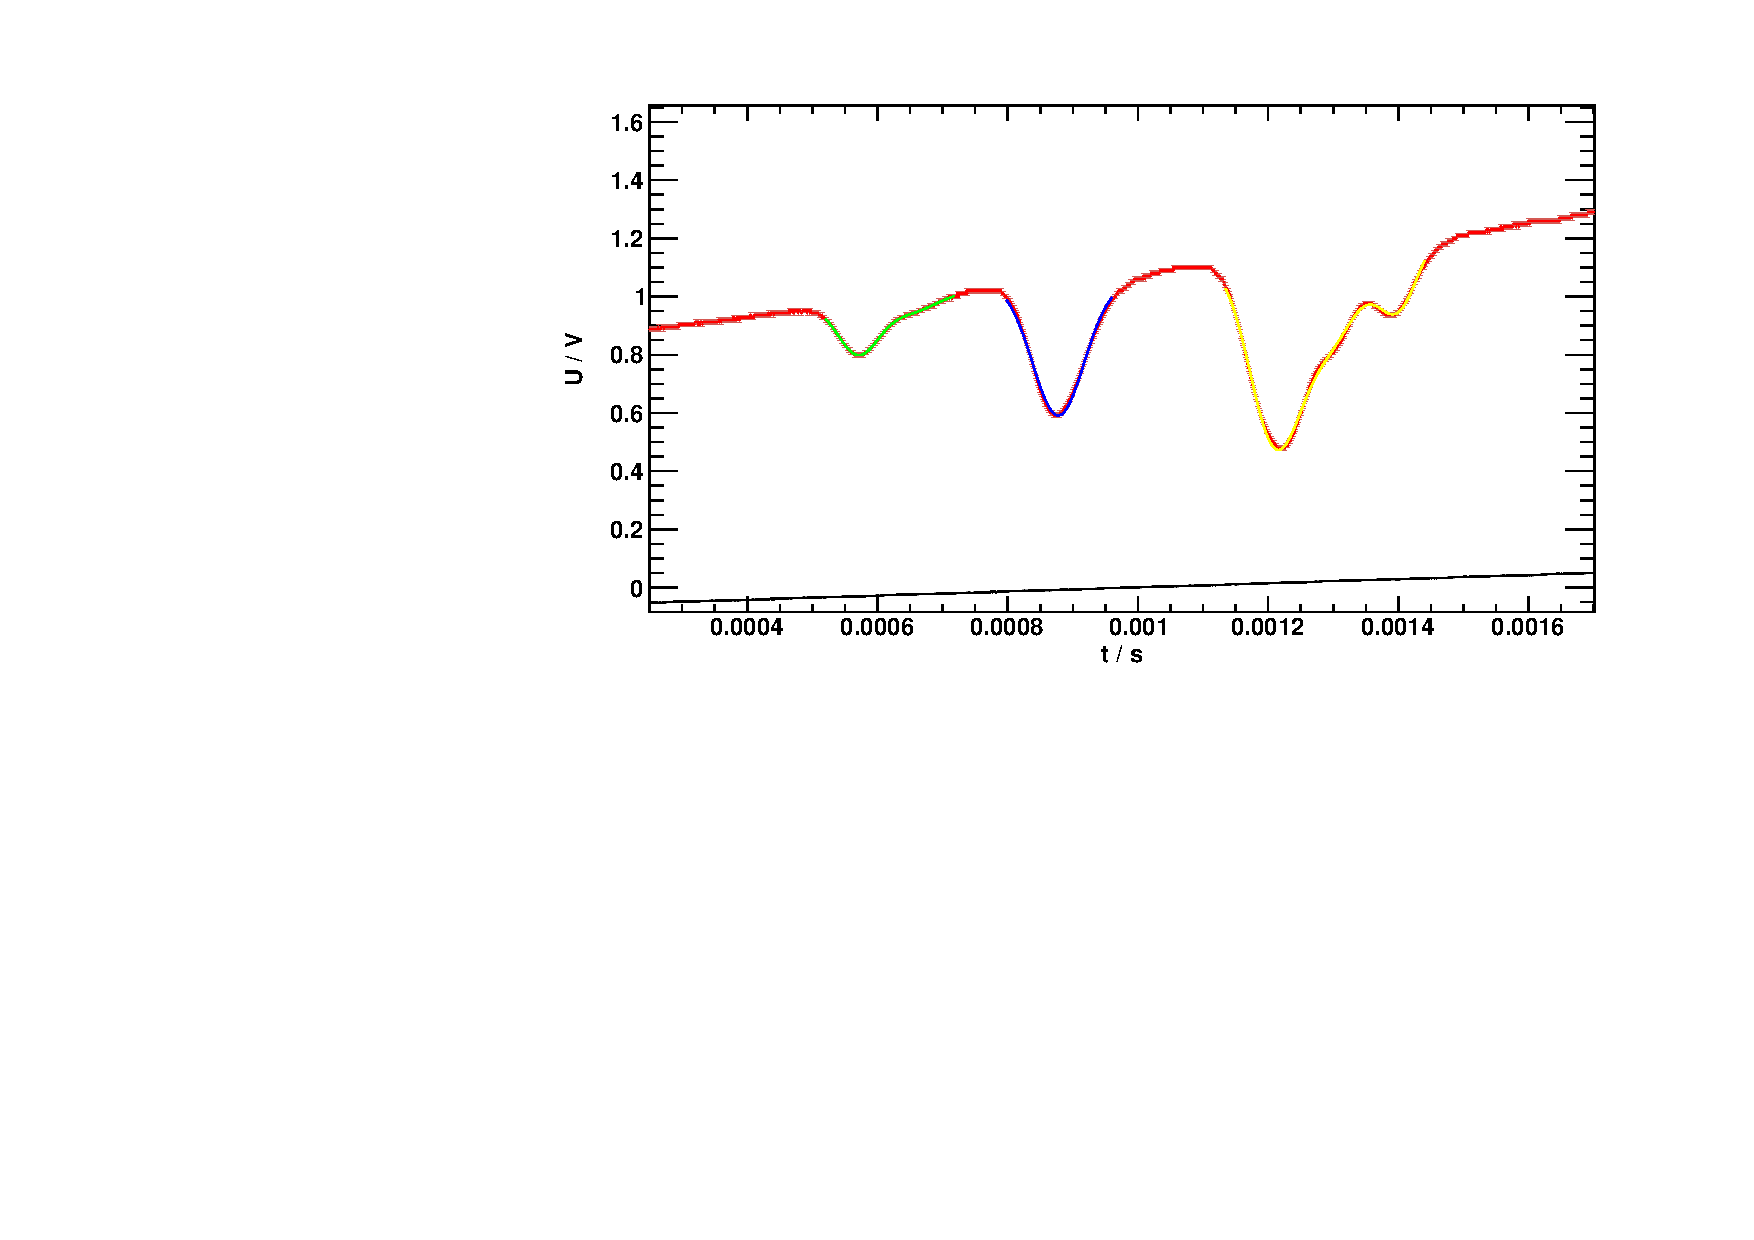
\includegraphics[width=\textwidth]{../img/part2/up-hfs_zoom_fit.pdf}  %TODO Better start params
  \caption{caption.}
  \label{img:hfs:fit:up}
\end{center}
\end{figure}

\subsubsection*{Berechnung des Spektrums}
Um aus den erhaltenen Positionen der Peaks nun eine absolute Frequenz zu berechnen, wird eine absolute Frequenz eines Peaks als Referenz 
benötigt. \\
großer Peak, Mittelwert aus beiden Linien
berechnung des spektrums 

\subsubsection*{Vergleich mit den Literaturwerten}
Tabelle mit Spektrumswerten (Literaturwert, aufsteigend, absteigend (eine Tabelle))
Gerade sollte Steigung 1 und Achsenabschnitt 0 Ghz haben

\begin{figure}[H]
\begin{center}
  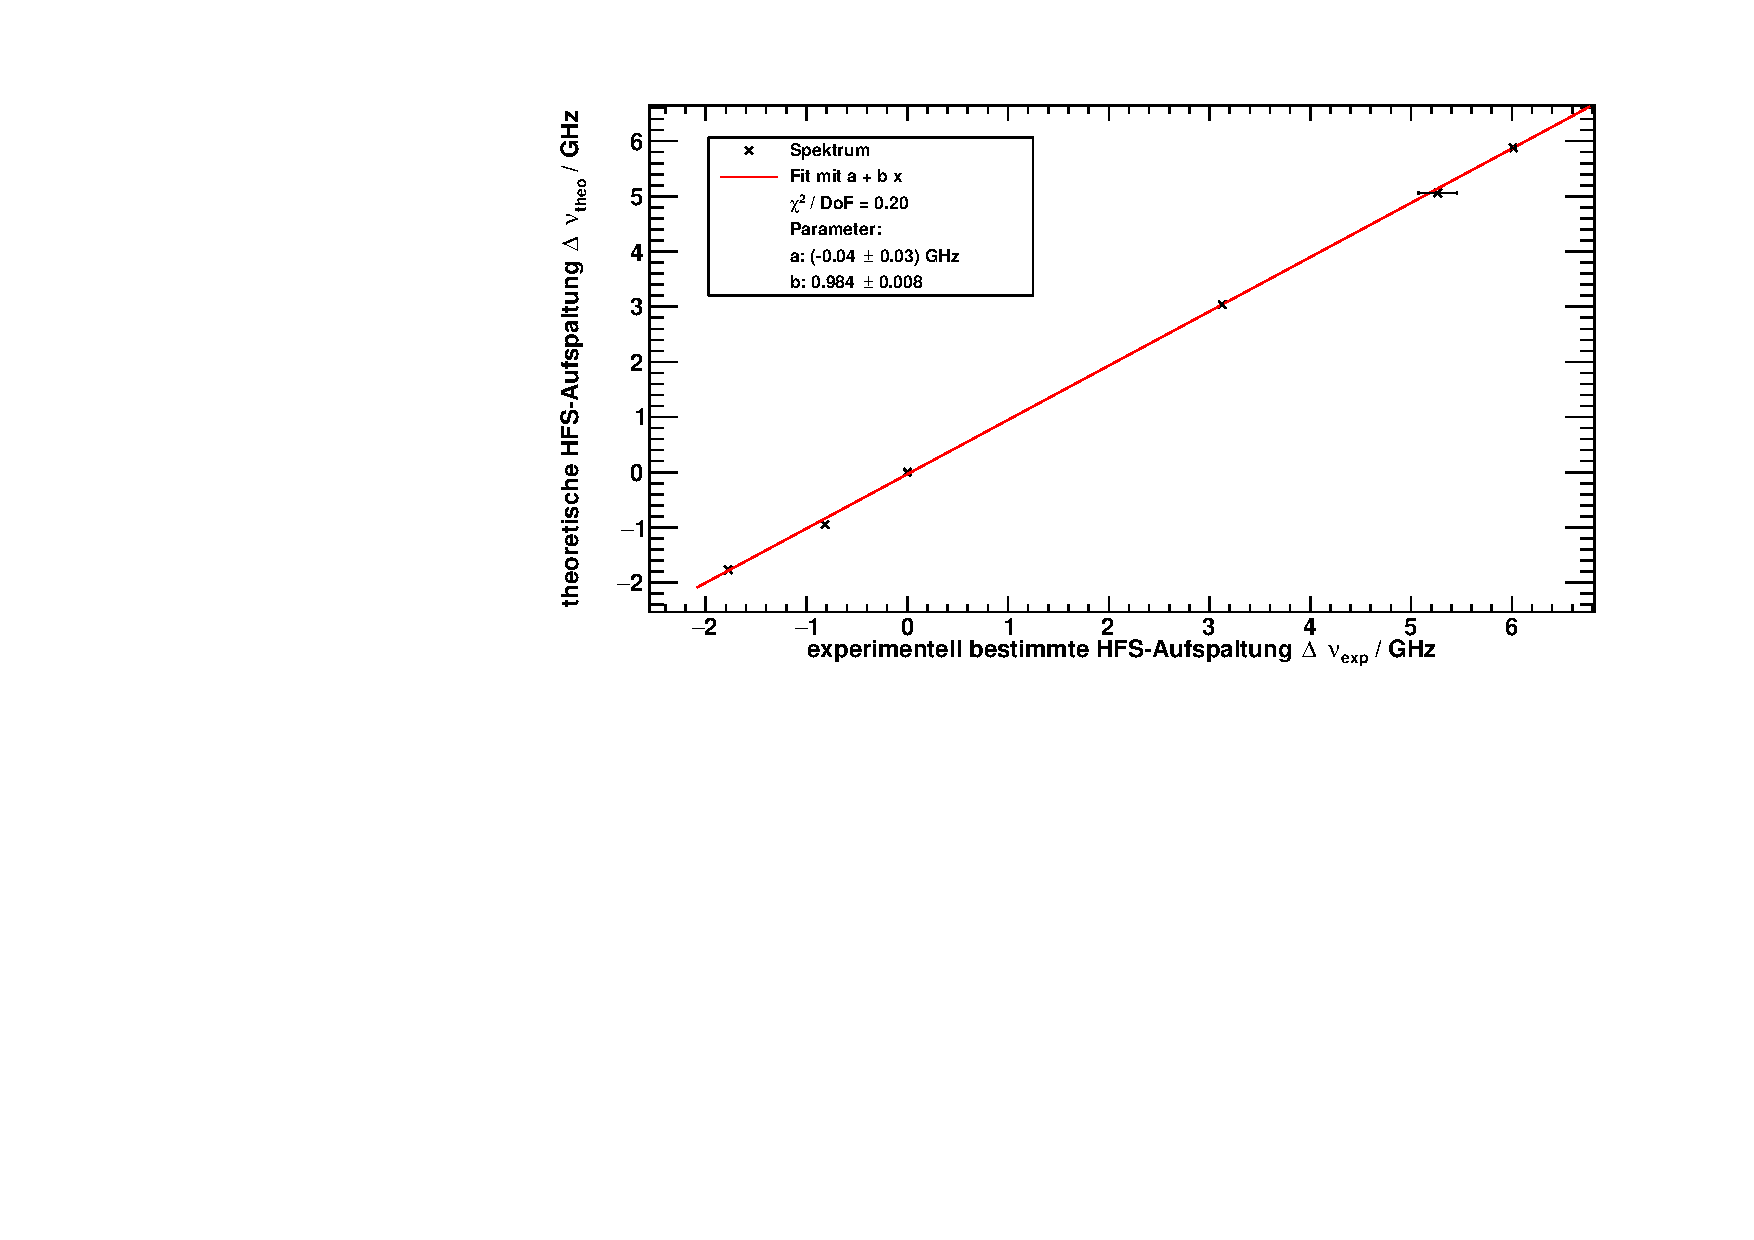
\includegraphics[width=\textwidth]{../img/part2/up-spectrum.pdf}
  \caption{caption.}
  \label{img:hfs:spectrum:up}
\end{center}
\end{figure}

\begin{figure}[H]
\begin{center}
  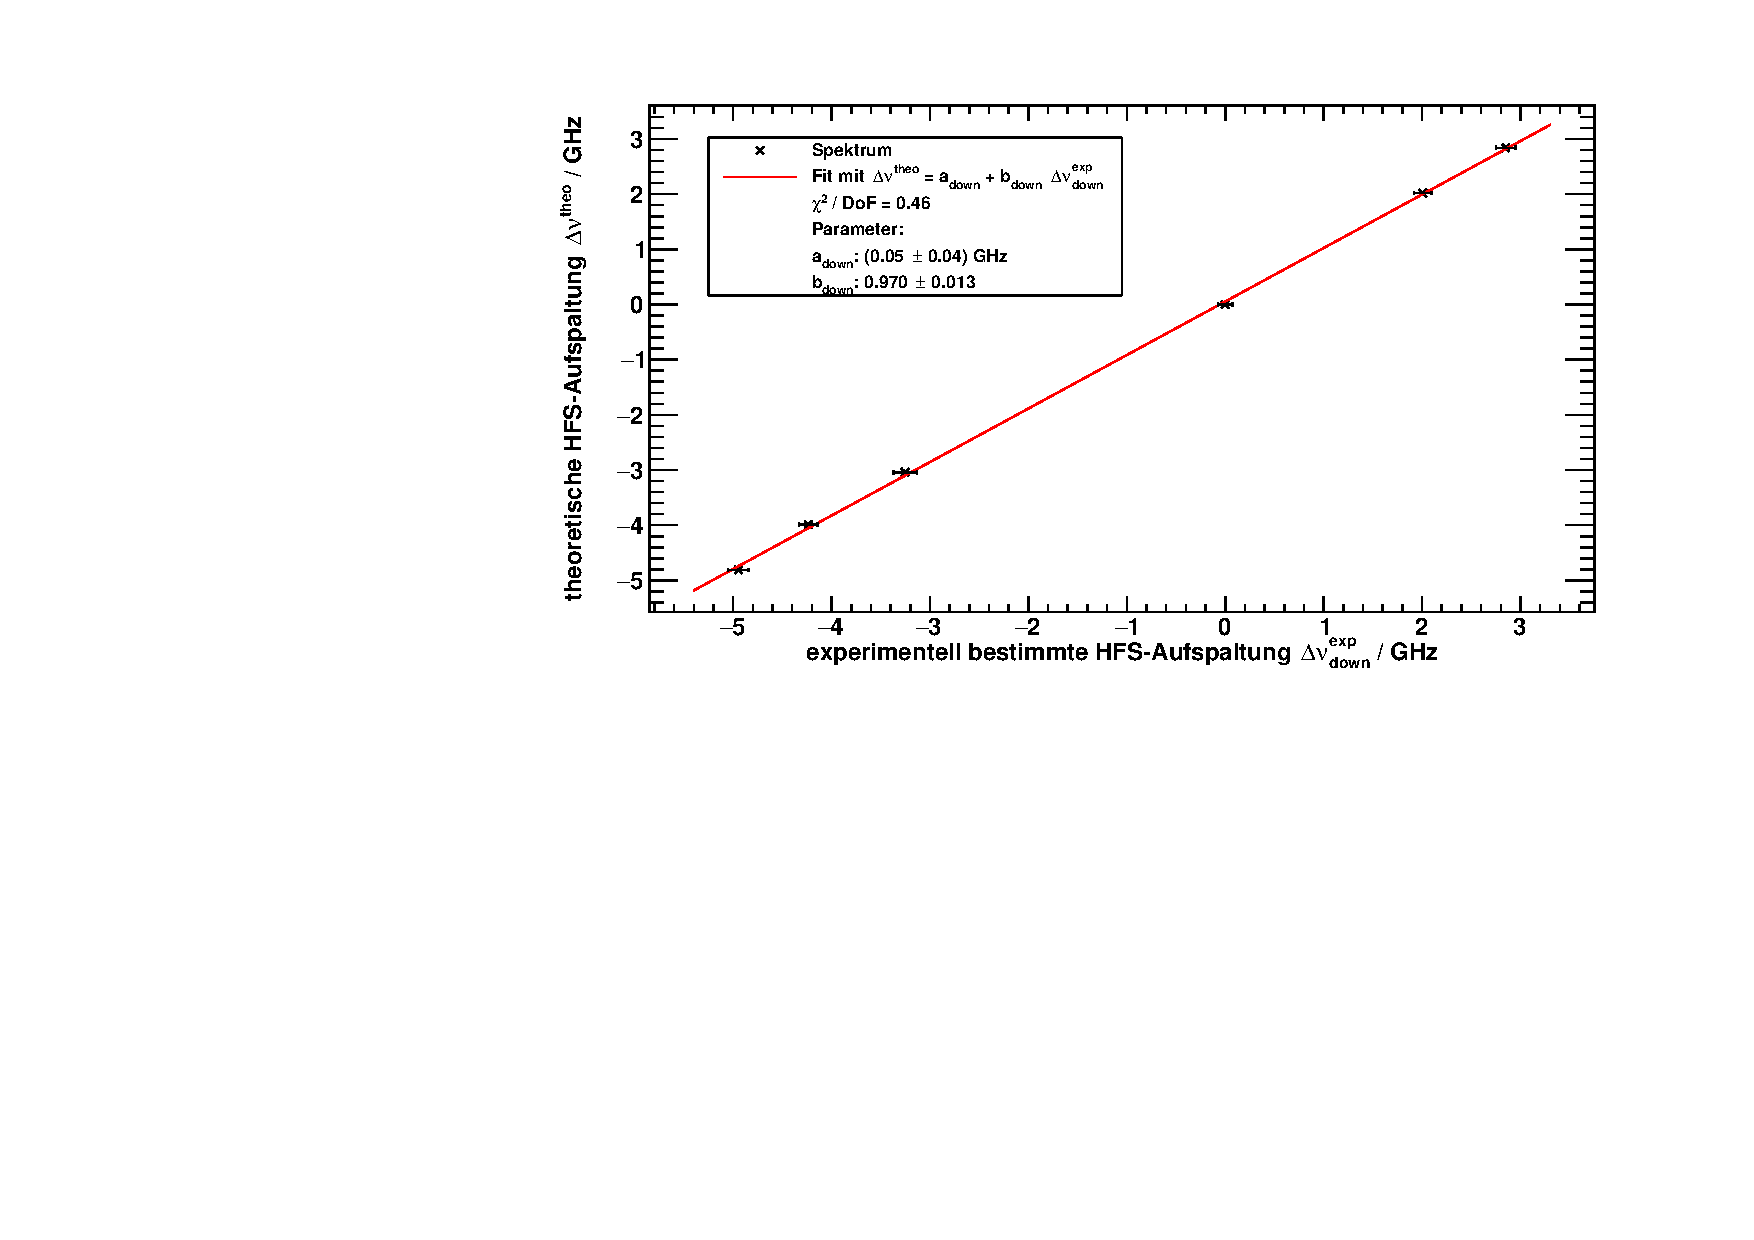
\includegraphics[width=\textwidth]{../img/part2/down-spectrum.pdf}
  \caption{caption.}
  \label{img:hfs:spectrum:down}
\end{center}
\end{figure}
